\documentclass[acmsmall, authorversion]{acmart}

\usepackage{fullpage}
\usepackage{amsmath}
\usepackage{url}
\usepackage{hyperref}
\usepackage{graphicx}
\graphicspath{ {images/} }
\usepackage{pgfplots}
\usepackage{fancyhdr}
\usepackage{blindtext}
\usepackage{mathtools}
\documentclass{amsart}
\usepackage{booktabs} % For formal tables
\usepackage{algpseudocode}
\usepackage[noend]{algpseudocode}
\usepackage[T1]{fontenc}
\usepackage[utf8]{inputenc}
\usepackage{tabularx,ragged2e,booktabs,caption}
\usepackage{float}


\usepackage[ruled]{algorithm2e} % For algorithms
\renewcommand{\algorithmcfname}{ALGORITHM}
\SetAlFnt{\small}
\SetAlCapFnt{\small}
\SetAlCapNameFnt{\small}
\SetAlCapHSkip{0pt}
\IncMargin{-\parindent}

\usepackage[justification=centering]{caption}


\pagestyle{fancy}
\fancyhf{}
\usepackage{lastpage}

\usepackage{fancyhdr}

\fancyfoot[C]{Page \thepage\ of \pageref{LastPage}}
\pagestyle{plain}

\makeatletter
\def\blfootnote{\xdef\@thefnmark{}\@footnotetext}
\makeatother

\usepackage[rightcaption]{sidecap}

\usepackage{wrapfig}

\renewcommand\shortauthors{Upadhyay, A. et al}

\title{Dependable Interference-Aware Time-Slotted Channel Hopping for Wireless Sensor Networks}

\author{Ankita Upadhyay}
\orcid{1234-5678-9012-3456}
\affiliation{%
  \institution{University of California, Santa Cruz}
}
\author{Rasool Tavakoli and Majid Nabi}
\orcid{1234-5678-9012-3456}
\affiliation{%
  \institution{Eindhoven University of Technology}
}





\begin{document}

\begin{abstract}
 Time-Slotted Channel Hopping (TSCH)'s main goal is to ameliorate communication reliability in Wireless Sensor Networks (WSNs). This is accomplished by reducing the medium access contention impact. Elements that comprise medium access contention impact include blocking of wireless links and multi-path fading. TSCH performs better than single-channel communications. However, ISM bands are affected by cross-technology interference which potentially affects TSCH-based WSNs performance. In-vehicle networks includes interference which is dynamic over time, which leads to non-guaranteed reliability throughout time. This article proposes an Enhanced version of the TSCH protocol together with a Distributed Channel Sensing technique (ETSCH+DCS) which aims to detects good quality channels to be utilized for communication. The channel quality is extracted using a distributed channel-quality estimation technique. The central technique uses Non-Intrusive Channel-quality Estimation (NICE) technique that detects energy interference in each timeslot's idle parts at the network coordinator location. 
\end{abstract}

\begin{CCSXML}
<ccs2012>
<concept>
<concept_id>10003033</concept_id>
<concept_desc>Networks</concept_desc>
<concept_significance>300</concept_significance>
</concept>
<concept>
<concept_id>10003033.10003034</concept_id>
<concept_desc>Networks~Network architectures</concept_desc>
<concept_significance>300</concept_significance>
</concept>
<concept>
<concept_id>10003033.10003039</concept_id>
<concept_desc>Networks~Network protocols</concept_desc>
<concept_significance>300</concept_significance>
</concept>
<concept>
<concept_id>10003033.10003068</concept_id>
<concept_desc>Networks~Network algorithms</concept_desc>
<concept_significance>300</concept_significance>
</concept>
</ccs2012>
\end{CCSXML}

\ccsdesc[300]{Networks}
\ccsdesc[300]{Networks~Network architectures}
\ccsdesc[300]{Networks~Network protocols}
\ccsdesc[300]{Networks~Network algorithms}

\keywords{wireless sensor networks, time-slotted channel hopping, in-vehicle wireless sensor networks, interference, dependable, channel quality estimation}

\blfootnote{Theoretical conference of submission: 16th ACM Conference on Embedded Networked Sensor Systems (SenSys 2018) \url{http://sensys.acm.org/2019/}} \blfootnote{Based article: Tavakoli, Rasool, et al. "Dependable interference-aware time-slotted channel hopping for wireless sensor networks." ACM Transactions on Sensor Networks (TOSN) 14.1 (2018): 3. \url{https://dl.acm.org/citation.cfm?id=3158231}}


\maketitle

\begin{abstract}
abstract
\end{abstract}



\printccsdesc



 \section{Introduction}

   Wireless Sensor Networks (WSNs) have numerous applications ranging from routing protocols to In-Vehicle Networks (IVNs). Their low power consumption properties along with their reconfigurable and flexible nature entail dependable communication as a result of high Quality-of-Service (QoS) specifications. This in turn calls for fulfilling requirements including availability, reliability, and maintainability which renders Time-Slotted Channel Hopping (TSCH) mode of the IEEE 802.15.4 \cite{tavakoli2015enhanced} standard to be a suitable contender for being utilized as the Medium Access Control (MAC) layer protocol. 
   
   TSCH, which is divided into time slots, utilizes Time-Division Multiple Access (TDMA) to allot a [timeslot, channel] tuple to every communication link within a network. TDMA allows channel accessibility for networks with shared mediums. TSCH accomplishes this by combining a channel hopping scheme with TDMA to ensure communication link accessibility. By using this method, TSCH secures link reliability in matters of interference and multi-path fading as well as ensures service availability in terms of wireless node access to the medium. Improvements are constantly being made to advance TSCH mesh networks performance and the uppermost TSCH layers. Nonetheless, more efforts need to be made in order to meet latency and reliability standards regarding IVNs. 
  \\ \indent To remedy this, we propose Enhanced Time-Slotted Channel Hopping (ETSCH), an improved version of the TSCH protocol \cite{de}. ETSCH extracts and filters channel quality by identifying energy detections in the idle sections of every time slot. NICE keeps the protocol static and conducts successive channel samplings. ETSCH also expands configuration packet based transmission reliability and uses low-noise channels for hopping by utilizing a sequence hopping method which enhances TSCH protocol reliability.This paper will present ETSCH+DCS mechanisms as well as an outline of TSCH protocol within an application scenario.  In addition, this paper will also include related work regarding low-power multi-channel communication and an overview of the proposed ETSCH+DCS method followed by a comprehensive performance analysis.

\section{Background} 
\subsection{Time-Slotted Channel Hopping}

TSCH is known as a MAC operating mode of the IEEE 802.15.4 standard \cite{chang} that supports industrial applications. TSCH is notorious for increasing communication dependability against multi-path fading and external interference. TSCH executes in timeslots where one timeslot takes a certain amount of time to transmit one packet. There is also the potential of collisions occurring. In order to avoid collisions, each link must be assigned to their respective timeslots. Multiple time slots are categorized as a \emph{slotframe}. Both ASN and Hopping Sequence List(HSL) allow nodes to compute each channel's timeslot through the equation:
\\
\begin{equation}
\centerline{\emph{Channel= HSL[(ASN + Channel Offset)$  \%|HSL|$]}}
\end{equation}

The absolute value of HSL indicates the number of channels in the HSL. Different links can include Different Channel Offset (DCO) which allow for parallel communication within a timeslot on a span of multiple channels. The upper layers in the protocol stack define the protocol stack standards which include the subset or the entirety of the HSL channels. This protocol helps mitigate intra-network collisions by instituting access to the node medium, thus improving network availability. Eradicating wireless link blocking and being able to hop over a span of multiple channels improves reliability as well. The Enhanced Beacon (EB) transmission is conducted through the network coordinators and can potentially be either aperiodic and/or periodic. EB also includes information from higher layer protocols for application-specific means.


\subsection{Application Scenario}
Wireless sensor networks that are in-vehicle can undergo  dynamic interference due to different wireless devices within the vehicle. These work in different sections of the 2.4GHz ISM band. Some applications that affect WSN activity include engine sensor monitoring, tire pressure monitoring, and window controlling. These aspects all include QoS despite being non-safety critical and must comply with the necessary wireless protocols. The amount of sensors and network size vary from vehicle to vehicle. For smaller vehicles, the sensor nodes are within each other's range and do not call for multi-hop communication while larger vehicles entail a larger network with different interference conditions and QoS requirements. WSNa inside vehicles should supply reliable multi-hop communication as there can be a non-uniform distribution among the various sensors within the wireless medium. For instance, a truck could experience interference among frequency channels from the vehicles on either end of the truck.

\section{Related Work}

Many protocols such as MAC operation encompass TSCH utilize channel hopping. Network communications are categorized by time slots which various network devices within synchronize. There is a set sequence-hopping pattern which aims to reduce multipath fading and interference caused by a narrow-brand. This allows improvements in network connectivity and reliability due to the rise of communication issues. The higher layers are then left to configure tasks including task scheduling and channel hopping lists. Network communication and reliability significantly improve as a result of task configuration and there is comprehensive function allocation as well \cite{jeon}.
One way to improve the channel hopping technique is to limit the used channels that we're sure are of strictly good quality \cite{de}. This is done by whitelisting. On the contrary, blacklisting is the method that detects channels of poor quality. Bluetooth uses Adaptive Frequency Hopping (AFH) to mitigate the impact of cross-technology interference by utilizing good channels. However, Bluetooth standards do not indicate how to detect bad or good channels. We propose two methods of detecting channel strength including Received Signal Strength Indication (RSSI) and Packet Error Rate (PER). Each aspect is selected by formulating an independent process that utilizes packet transmission status (packet acknowledgement status) and Clear Channel Assessment (CCA) failures on that particular channel \cite{els}.

\section{Enhanced Time-Slotted Channel Hopping with Distributed Channel Sensing}

\subsection{Overview}
ETSCH entails choosing a low-noise subset which is then inputted into the channel hopping algorithm after being filtered and examined. The white listing is centralized and each node exists within the coordinator communication range. Each node can have a data link scan between them by utilizing the given white listed channels. Between each node exists  three components that follow a mesh topology. Fig. 1 breaks down the components and depicts how the DCS technique in the protocol stack shows the TSCH slot frame and structure. These components exist and run in the idle section of the time slots which renders their execution useless. Algorithm 1 depicts the component wire frame. Every wireless node within the network includes a DCS component that identifies the channel status and relays the information to the coordinator in the network. Fig. 1 demonstrates NICE running in parallel with TSCH on the MAC layer to examine the channel quality. NICE has protocol EDs which measure the frequency channel quality. An ED estimates the signal power in the channel bandwidth and takes eight symbol periods (i.e., 128$μs$). There are bounds that are linearly mapped and measured in dB \cite{chang}. The NICE technique is depicted in the first part of Algorithm 1.

\begin{figure*}[t]
\begin{multicols}
\centering
    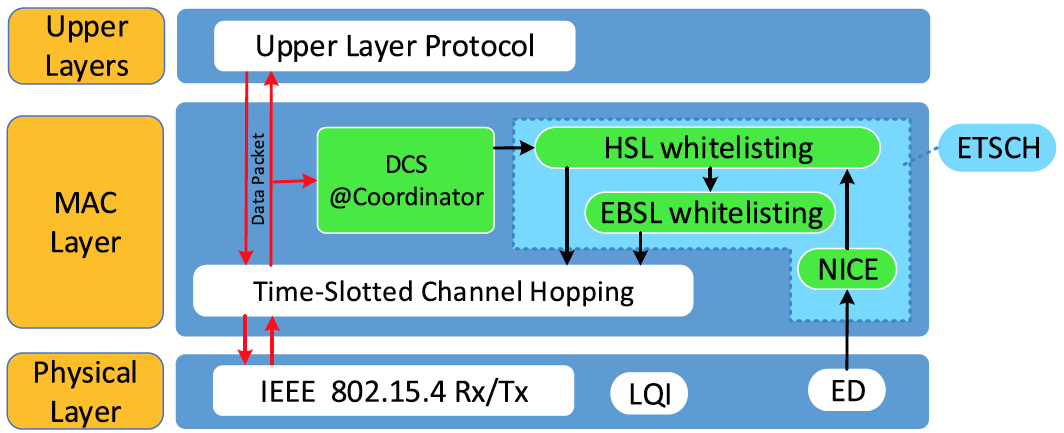
\includegraphics[width= \textwidth]{mac1.png}
    \caption{ETSCH+DCS components in the coordinator node.}
\end{multicols}
\end{figure*}

\begin{figure*}[t]
\begin{multicols}
\centering
    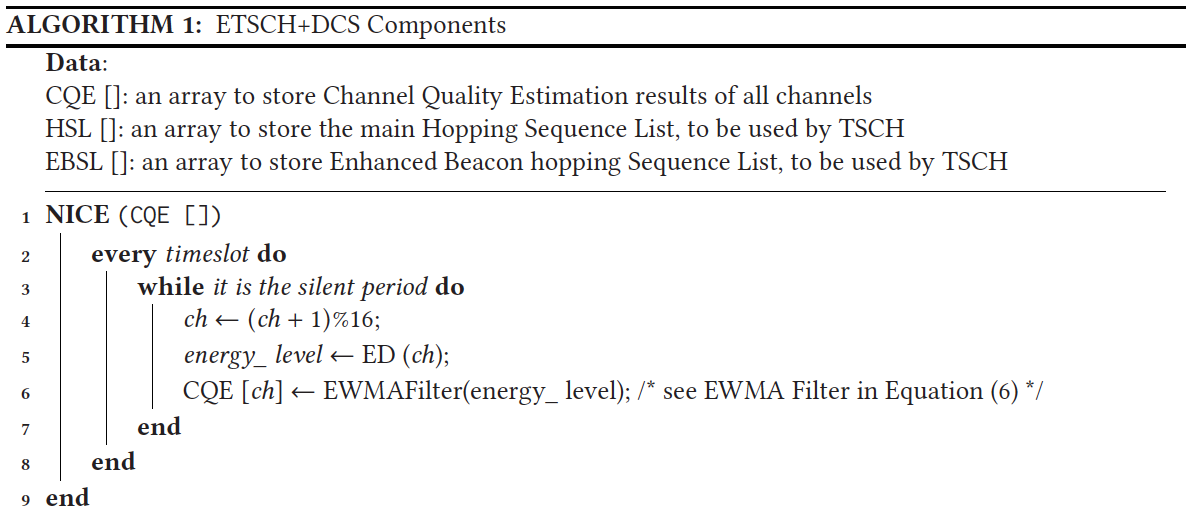
\includegraphics[width= \textwidth]{algofinal.png}}
\end{multicols}
\end{figure*}

\subsection{Non-Intrusive Channel-quality Estimation}

In order for there to be a noise level estimation from a frequency channel, there should not exist any network transmissions in that time period. NICE utilizes various frequency channels with minimal protocol-based bandwidth cost to the protocol \cite{gomes}. We observe the NICE method execution and the TSCH communication diagram.  Synchronized time slots then dictate node communication. A receiver node must know the beginning of the sender's channel time slot so they switch the radio on and conduct transmission by paying attention to the medium. The nodes can contain lagging and clock drifts which renders the synchronization process to be continuous in order to consider phase differences within the time slot. Because of clock drift between the nodes, the synchronization process needs to be continuously performed to keep the nodes synchronized. To compensate an amount of timeslot phase differences caused by clock drifts, TSCH defines a diagram for timeslots shown in Figure 2. The timeslot duration, \textit{macTsTimeslotLength}, is long enough for transmission of a maximum size packet and its corresponding ACK. There is an offset \textit{macTsRxOffset} at the beginning of a receiver’s timeslot before it starts listening to the medium. This \textit{Rxoffset} prevents interference from other nodes in the network.

\begin{figure*}[t]
\begin{multicols}
\centering
    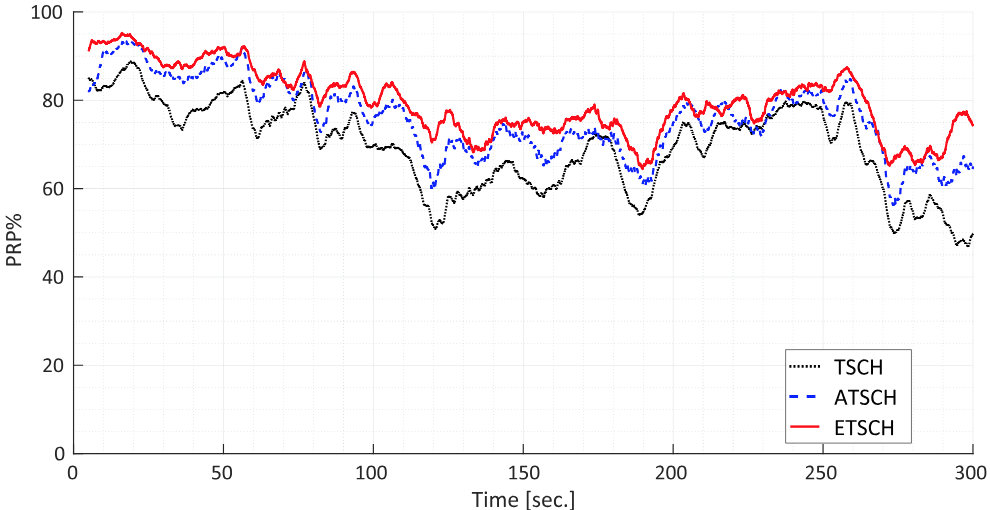
\includegraphics[width= \textwidth]{redblack.png}} 
    \caption{Effect of the Mixed lifelike interference on the IEEE 802.15.4 channels and performance of different mechanisms under this interference, extracted by simulations.}
\end{multicols}
\end{figure*}

The MAC is defined for a sender. It then performs a Clear Channel Assessment in order to prevent packet transmission if the channel is busy. When the receiver starts listening to the channel for a reception in a timeslot, it waits for a designated time period before it responds. If the transceiver cannot identify any packet preamble in this period, then the receiver considers this situation as a packet transmission failure and ceases to listen further. The values of these parameters are defined so that the MAC offset and the wait time is larger than the MAC offset. This renders the communication successful if the receiver is ahead of the sender for what would be the maximum difference of these two values. Some other timings such as the ACK transmission timings are defined in the protocol as well. We investigate different cases in order to identify the maximum allowed phase difference for default values. Considering the fact that the coordinator of a wireless network is the main source of synchronization, the device won't be allowed to communicate with a device that starts backward $100μs$ after the coordinator. To enable bidirectional transmission between each pair of nodes in the network, the forward and backward timeslot phase differences should be less than $TMaxbackward=TMaxforward=450μs$. This value is extracted by considering the required time for PHYSHR detection at receiver, which should happen before the end of the listening period at receiver. This means that the employed timeslot synchronization method should guarantee the synchronization loss to be less than these values to have a connected mesh network \cite{els}. Therefore, from the coordinator perspective, for the time period within each timeslot, there is a possibility of packet transmissions by some nodes in the previous timeslot. Also, there is the possibility that some nodes start packet transmissions ahead of the coordinator. Considering these possibilities, there will be no packet transmission in the network for the designated silent period.

\subsection{Distributed Channel Sensing}

Due to synchronization loss caused by clock drifts, it is impossible to determine the silent period at non-coordinator nodes. Thus, we cannot use NICE to extract the quality of the channels in non-coordinator nodes. However a third hop interferer, which is hidden from the coordinator, may generate interference for some of the other nodes. Therefore, we employ a distributed channel quality estimation technique called DCS to work together with NICE as the interference detection block of ETSCH. The overhead of such a sensing technique should be taken into consideration. Using channel EDs at non-coordinator nodes \citep{de} leads to extra power consumption that is a negative point in battery-powered wireless nodes. We take advantage of CCA and packet reception status, which are already available and defined in the protocol, as two parameters representing conditions of each communicating channel. All of these parameters give an estimation about the channel quality at the point of the measuring/receiving node. This provides enough information about the existence of interference at each node. The only limitation of using these parameters is that they only give information about the condition of the channels that are being used for communications. In other words, the condition of blacklisted channels is not extractable using these parameters. However, this is not an issue in ETSCH, since when a channel is detected as a bad-quality channel and is blacklisted, NICE still measures its quality and updates the assigned CQE to it. Therefore, if the coordinator realizes that the quality of a blacklisted channel is better than a used channel, there is a chance for that channel to be used for communications again.

\subsection{Channel Whitelisting}
Whitelisting is performed periodically by the coordinator of the network to select a subset of good-quality channels as the HSL for the TSCH protocol. The results of NICE and DCS, which are combined as a unique CQE array, are used as the input the given algorithm. There are different ways to perform whitelisting. In order to choose a proper technique, a few constraints should be taken into account to do whitelisting for a TSCH network. First, if the whitelist size is not prime to the slotframe size, each timeslot only touches a subset of the channels in the HSL, not all of them. This will cause a  chance of failures for different timeslots over time. Thus, using a variable size whitelist with all possible whitelist sizes could potentially cause problems. Furthermore, if an allocated link to a timeslot experiences persistent multi-path fading on a channel, its packet error rate will be increased. We use a fixed size whitelist in this work, but it is also possible to use a variable size whitelist with sizes that are prime to the slotframe size. It should be considered that smaller whitelist sizes reduce the maximum number of channel offsets that can be utilized. This causes internal interference and packet losses. Accordingly, smaller whitelist sizes reduce the number of parallel communications that can be established at one timeslot and also the overall throughput of a TSCH network. In threshold-based approaches, the number of channels with a better quality than a specified threshold may be very low. Thus, it may not provide enough channels to meet a specific whitelist size. On the other hand, by using the NICE and DCS techniques, we assigned qualities to all of the channels and we can use these values to sort them. Therefore, we use a ranking technique to select a fixed number of best quality channels as the HSL for ETSCH \cite{gomes}. The resulting shuffled HSL is used by the TSCH protocol for the hopping procedure.

\section{Performance Evaluation}
\subsection{Setup}
To evaluate the performance of ETSCH, our implementation follows default TSCH timings, which is defined in the standard. We also exploit some controlled noise generators using Atmel motes, which is an implementation of the IEEE 802.15.4 MAC kit. Because of different channel setups in different wireless standards, networks may observe interference on multiple adjacent channels from a coexisting wireless technology (e.g., Wi-Fi). To mimic this real situation in our setup, each noise generator provides controlled interference by transmitting dummy packets on a pair of adjacent IEEE 802.15.4 channels. To implement this mechanism, a noise generator transmits a short packet on a channel and immediately hops to the paired adjacent channel. This process is done continuously to generate interference on both the paired adjacent channels only by one noise generator. Furthermore, each noise generator can be programmed to hop to different pairs of adjacent channels within predefined periods and using a predefined sequence. The DCS technique is proposed for situations where there is an interference source around the network that is hidden from the coordinator. Actually, when there is no hidden interference source,the DCS technique has no effect on the channel whitelist, and whitelisting only follows the output of NICE. Based on this, we define two evaluation sets to study the performance of the ETSCH technique without any interference hidden from the coordinator and the ETSCH+DCS technique under existence of hidden noise. In the first evaluation set, we compare the performance of ETSCH with ATSCH and basic TSCH using experiments and simulations. The experiments area summary of the results of \cite{xia} in which we used different levels of interference dynamism to evaluate the agility of the available channel sensing techniques. In addition to the lab experiments, performance of the ETSCH technique is evaluated under realistic in-vehicle scenarios, using simulations and real-world interference datasets.
For the second evaluation set, we use experiments and focus on the performance evaluation of the DCS technique in the presence of hidden interference that is not detectable by NICE. Because DCS is an additional technique on top of ETSCH, we also perform the same experiments for ETSCH as well as TSCH to compare the results.

\subsection{ETSCH Performance Evaluation}
This subsection evaluates the performance of ETSCH (skipping the DCS technique) in comparison with other channel quality estimation technique called ATSCH and also the TSCH protocol. Wireless interference is the main source of packet errors in urban networks, whitelisting can reduce this negative effect by using good-quality channels. The level and also dynamic nature of interference can affect the performance of the whitelisting technique. To test the performance of ETSCH, we use experiments with controlled noise generators as well as simulations with real-world in-vehicle interference on IEEE 802.15.4 channels. The number of noise generators used with respect to interference levels is recorded in Table 1. We try different interference scenarios with different levels and dynamism of interference for the network under test as seen in Fig.3. We investigated various metrics to evaluate the performance of the proposed techniques. Packet Reception Probability (PRP) is the probability of one successful packet transmission for given noise power during transmission of each bit of that packet in simulations. PRP is a probabilistic value that is extracted based on the signal to noise ratio. On the other hand, Packet Reception Ratio (PRR) is the number of packets that are successfully received at the receiver node over the total number of packets transmitted by the sender node, extracted from the experiments. Both metrics reflect the quality of the links. The length of burst packet losses is the number of consecutive packets losses over a link and shows the time duration of link level disconnections. This metric is important for many applications to avoid long disconnections, as they required continuity of correct service overtime. The maximum of this metric shows the worst-case latency of a link in a TSCH network if the number of re-transmissions is infinite. 

\subsubsection{Lab Experiments, Setup, and Analysis.}
We use a mesh TSCH network with seven de-vices and one PAN coordinator. We use a wider area for our experiments, compared to an in-vehicle network in a truck. This is because due to obstacles (such as body of the car and passengers) in an in-vehicle testbed, quality of links are normally lower than an office workspace. 

   \begin{table}[H]
   \caption{Interference Scenarios and Behavior \label{interference}}
                    
                    \begin{tabular}{ |p{5.2cm}||p{5.2cm}| }
 \hline
 \multicolumn{2}{|c|}{Interference Scenarios} \\
 \hline
 \emph{Scenario} & \emph{Behavior of NG(s)} \\
 \hline
 No interference   & no controlled NG    \\
 \hline
 Low interference &  noise on 2 channels (1 NG), hop every 20s to new channels  \\
 \hline
 Medium interference & noise on 6 channels (3 NGs), hop every 20s to new channels\\
 \hline
 High interference    & noise on 6 channels (3 NGs), hop every 5s to new channels\\
 \hline
\end{tabular}
\end{table}

\begin{figure*}[t]
\begin{multicols}
\centering
    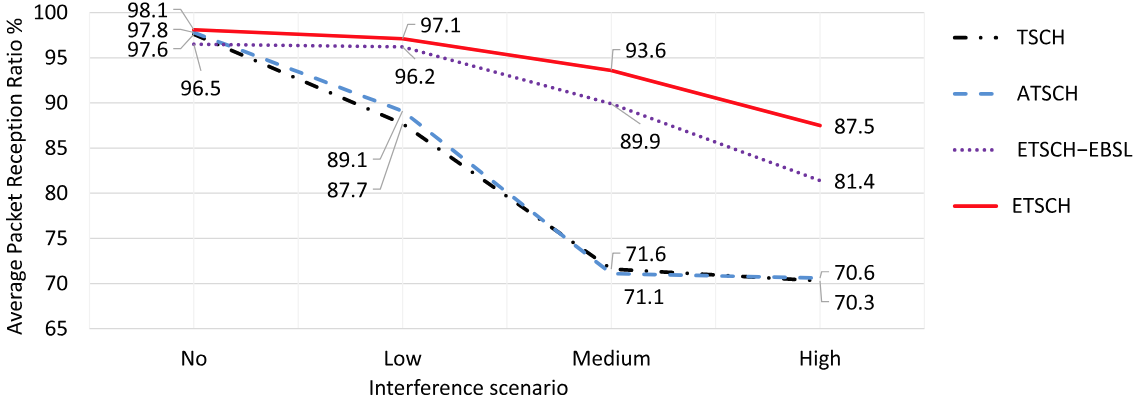
\includegraphics[width= \textwidth]{redblue2.png}}
    \caption{Average achieved PRR of different mechanisms for different interference scenarios.}
\end{multicols}
\end{figure*}

Instead of obstacles, we use longer distances between motes to reduce the link qualities in the experiments. We ran the experiments using a complete ETSCH with NICE and EBSL, and also a reduced version of it without the EBSL (Enhanced Beacon Sequence List), called ETSCH–EBSL (ETSCH minus EBSL) in this section for ease of reference. ETSCH–EBSL uses the basic hopping sequence list (all 16 channels) to transmit EBs. This allows us to investigate the impact of the EBSL on the performance of the network. We also implemented ATSCH (Advanced Time Slotted Channel Hopping) \cite{de} on top of our TSCH implementation to use it for our performance evaluations. Slotframes of size $S=11$ are used in the experiments to be prime to the hopping sequence. The first timeslot is allocated to EB transmission by the coordinator, 7 other timeslots each is allocated to one of the devices to transmit a packet of 100 bytes, and the three last timeslots are idle. As ATSCH needs two more timeslots per slotframe to perform EDs, we use two of the three idle timeslots for it. Each experiment lasts 6,000 slotframes, and thus each mote broadcasts 6,000 packets in an experiment. All motes listen to all the timeslots for packet reception from other motes. Doing this, we can extract the quality of all available links in the network, as we build a full mesh network. We run a number of experiments with different values to find a proper value. A value of around 0.1 was found to have the best results. We use values of a power of 2 for all the used coefficients, so that calculations can be simplified using bitwise shift; this minimizes the processing overhead on the sensor nodes. As seen in Fig. 3 and Fig. 4, we consider four interference scenarios in our experiments as follows: high, medium, low, and no interference. In the no interference scenario, we run the experiments without any controlled noise generator to see the cost of periodic HSL changes on the performance of our mechanism as depicted in Table 1. An in-vehicle network in a moving car constantly experiences interference from different sources (e.g., Wi-Fi networks). Assuming that each interference source is visible over a range of up to 50m, and this car moves with a speed of 36km/h, each noise source would be visible for 5s. Our high-interference scenario models this kind of interference when there are three interference sources visible at any time, which each generate interference on two IEEE 802.15.4 channels. This scenario simulates the situation that a car moves into the range of a new interference sources (e.g., a Wi-Fi network) every 5s. For the medium interference scenario, we consider lower mobility of IVNs, which leads to increasing the visibility duration of each interference source. Thus, we have lower dynamism of interference in this scenario. In the following, we analyze the results of this experiment set for different interference scenarios. Both versions of ETSCH provide better PRR on average in comparison to TSCH and ATSCH, when the network experiences dynamic interference. This shows the effect of highly adaptive channel quality estimation that is realized by NICE, which selects the best quality channels for hopping \cite{gomes}. Also, ATSCH performs almost the same as basic TSCH. Therefore, it can only deal with very low dynamic interference, and it cannot detect and follow the highly dynamic interference (that exists in in-vehicle networks). This leads to increasing packet losses when noisy channels are also selected to be used in the HSL.


\begin{figure*}[t]
\begin{multicols}
\centering
    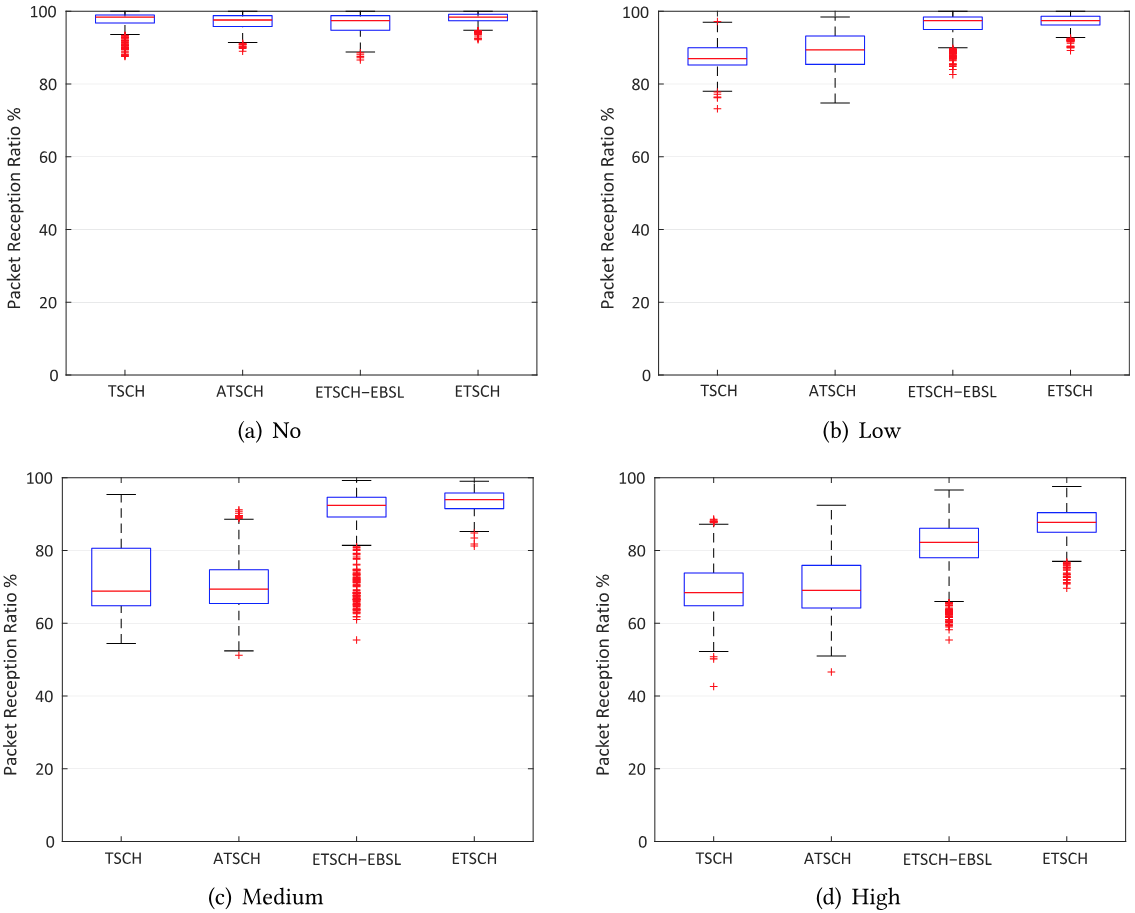
\includegraphics[width= \textwidth]{fourgraphs2.png}
    \caption{PRR distribution of incoming links to different nodes over windows of 500 transmissions for different mechanisms in hidden interference setup.}
\end{multicols}
\end{figure*}


\section{Conclusions}
This article proposes ETSCH+DCS, a mechanism on top of the TSCH protocol that uses a combination of a central and a distributed channel-quality estimation technique. This mechanism extracts the quality of different wireless channels to select the channels with the lowest interference as the hopping sequence list to improve the performance of the TSCH protocol. The central channel measurement technique, NICE, operates at the coordinator of the network and proactively measures the spectrum energy in the idle part of each timeslot, when all the nodes in the network are silent. The energy sampling results are used to assign qualities to wireless channels. The distributed technique is performed by all the nodes in the network and uses the CCA results together with packet reception status to estimate the noise level on each channel. To use the packet reception status as a sign of interference on the communication channel, it is proposed to send a dummy packet with the shortest possible MAC header, when there is no packet available from the application layer. Based on the TSCH communication diagram, it can be shown that transmitting a small packet consumes less overall energy than not sending a packet, because of reduced idle listening. The results of the centralized and distributed channel quality estimation techniques are used to assign a quality factor to each channel. Using these qualities, channels with better qualities are periodically selected as the hopping sequence list of TSCH. ETSCH+DCS allots a small secondary hopping sequence list (EBSL), that consists of the best quality channels, to disseminate periodic EBs. These EBs contain control information of the network such as the HSL. Only one field of the EBSL is updated per period, and thus the rate of EB losses in the network is reduced compared to using the regular HSL for broadcasting EBs. Experimental and simulation results show that ETSCH with NICE and EBSL provides higher packet reception ratios and lower length of burst packet losses compared to the plain TSCH protocol and another related work called ATSCH. Experiments also show that the DCS technique can detect existing interference in parts of the network that is not detectable by the centralized NICE technique, thus increasing the PRR in those scenarios.

    

\bibliographystyle{unsrt}
\bibliography{main.bib}
  
\end{document}

